\documentclass[12pt]{article}
\usepackage{graphicx}
\usepackage{geometry}
\usepackage{listings}
\geometry{a4paper, margin=1in}

\title{C-Lab: COP290 Project}
\author{Vihaan Luhariwala(2023CS10151) \\ Arinjay Singhal(2023CS10041) \\ Tejaswa Singh Mehra(2023CS10133)}
\date{}

\begin{document}

\maketitle


\section*{Design Decisions}

Our design focuses heavily on optimizing space throughout the implementation. 

\subsection*{ParsedInput Data Structure}

The \texttt{ParsedInput} structure is central to our design. It employs a union to consolidate different expression types—such as simple values, arithmetic expressions, range functions, and sleep operations—into a single structure. This union-based approach ensures that only the memory required for the active expression is allocated, rather than reserving space for all possible fields. Additionally, our design uses \texttt{16-bit int} types for row and column indices and encodes a cell's location within a single integer (using the first 16 bits for the row and the second 16 bits for the column). This allows us to use a single int to represent both a constant and a cell.

\subsection*{Input Parsing}
Input parsing is implemented manually without the overhead of regular expressions. This method:
\begin{itemize}
    \item Separates cell references from the associated expressions.
    \item Handles multiple expression types (arithmetic, range-based functions, direct references) with simple, efficient logic.
\end{itemize}

\subsection*{Dependency Management}
Dependency management is addressed in the \texttt{graph\_checker.h} file. Each cell maintains a dynamically allocated linked list (using the \texttt{Node} structure) to track its dependencies. Key functions include:
\begin{itemize}
    \item \texttt{add\_dependency}: Dynamically allocates nodes only when a new dependency is introduced.
    \item \texttt{free\_from\_list} and \texttt{free\_parents}: Ensure that obsolete or unwanted dependencies are promptly removed and memory is freed.
\end{itemize}
This on-demand allocation strategy means that only active dependencies consume memory, thereby optimizing space usage across the entire spreadsheet.

\section*{Challenges Faced}

Our design, though focused on minimizing space usage, encountered several challenges during implementation.

\subsection*{Memory Optimization and Avoiding Leaks}
The program relies heavily on dynamic memory allocation, particularly for maintaining the spreadsheet and dependency management routines. However, it introduces the challenge of optimizing space as maintaining a 999x18278 size spreadsheet requires a lot of memory, especially given the need for a variety of additional data structures to maintain formulae and dependencies.


\subsection*{Issues with Union Usage in \texttt{ParsedInput}}
The \texttt{ParsedInput} structure uses a union to consolidate various expression types (numeric values, arithmetic operations, range functions, sleep operations) into a single, compact data structure. A value can be a constant or a cell expression.

However, this approach has its pitfalls:
\begin{itemize}
    \item Data misinterpretation may occur if the active type is not correctly maintained, leading to potential bugs during evaluation.
    \item Updating a cell's expression requires careful handling to ensure that the union's content is properly refreshed, which increases the complexity of debugging.
\end{itemize}

\subsection*{Dependency Graph Management}
The dependency management system, detailed in \texttt{graph\_checker.h}, uses dynamically allocated linked lists to track cell dependencies. Critical functions include:
\begin{itemize}
    \item \texttt{add\_dependency}: Allocates nodes only when a new dependency is detected, conserving space.
    \item \texttt{free\_from\_list} and \texttt{free\_parents}: Ensure that outdated or unwanted dependency nodes are promptly removed and deallocated.
\end{itemize}
Managing these dynamic lists efficiently, especially during frequent updates and cycle detection (via the stack-based method in \texttt{mark\_dirty}), required balancing performance with meticulous memory management to avoid leaks.



\section*{Program Structure}

\subsection*{Core Modules}
\begin{itemize}
    \item \textbf{main.c}: Manages initialization, command parsing, and overall program flow.
    \item \textbf{initializer.h}: Stores data structures and basic functions which are crucial for initializing the program.
    \item \textbf{input\_parser.h}: Converts user inputs into structured formats for evaluation.
    \item \textbf{graph\_checker.h}: Manages dependency relationships, detects cycles, and ensures consistency.
    \item \textbf{input\_processing.h}: Processes commands and updates spreadsheet values.
    \item \textbf{display\_sheet.h}: Handles scrolling, display toggling, and viewport rendering.
    \item \textbf{testsuite.c}: Automates validation of functionality, edge cases, and error handling.
\end{itemize}

\subsection*{Key Data Structures}
\begin{itemize}
    \item \textbf{Cell}: Represents a single spreadsheet cell, including its value, parsed input, and dependencies.
    \item \textbf{ParsedInput}: Encodes user commands and formulas into a structured format for evaluation.
    \item \textbf{Node}: Represents a dependency relationship between cells in the graph.
\end{itemize}

\section*{Test Cases}

\begin{itemize}
    \item Detect cycles in cell dependencies, e.g., \texttt{A1 = B1 + A1}.
    \item Test arithmetic operations (\texttt{+, -, *, /}), including edge cases like negative values and zero.
    \item Validate division by zero sets the result to an error state.
    \item Evaluate range-based functions: \texttt{SUM, AVG, MIN, MAX, STDEV}, including empty and invalid ranges.
    \item Test the \texttt{SLEEP} function for both positive and negative values.
    \item Verify the program handles maximum dependency limits without crashing.
    \item Assign and reassign cells with dependencies (e.g., formulas involving \texttt{SLEEP}) to ensure proper updates.
\end{itemize}


\newpage

\section*{Diagram}
\begin{figure}[h!]
    \centering
    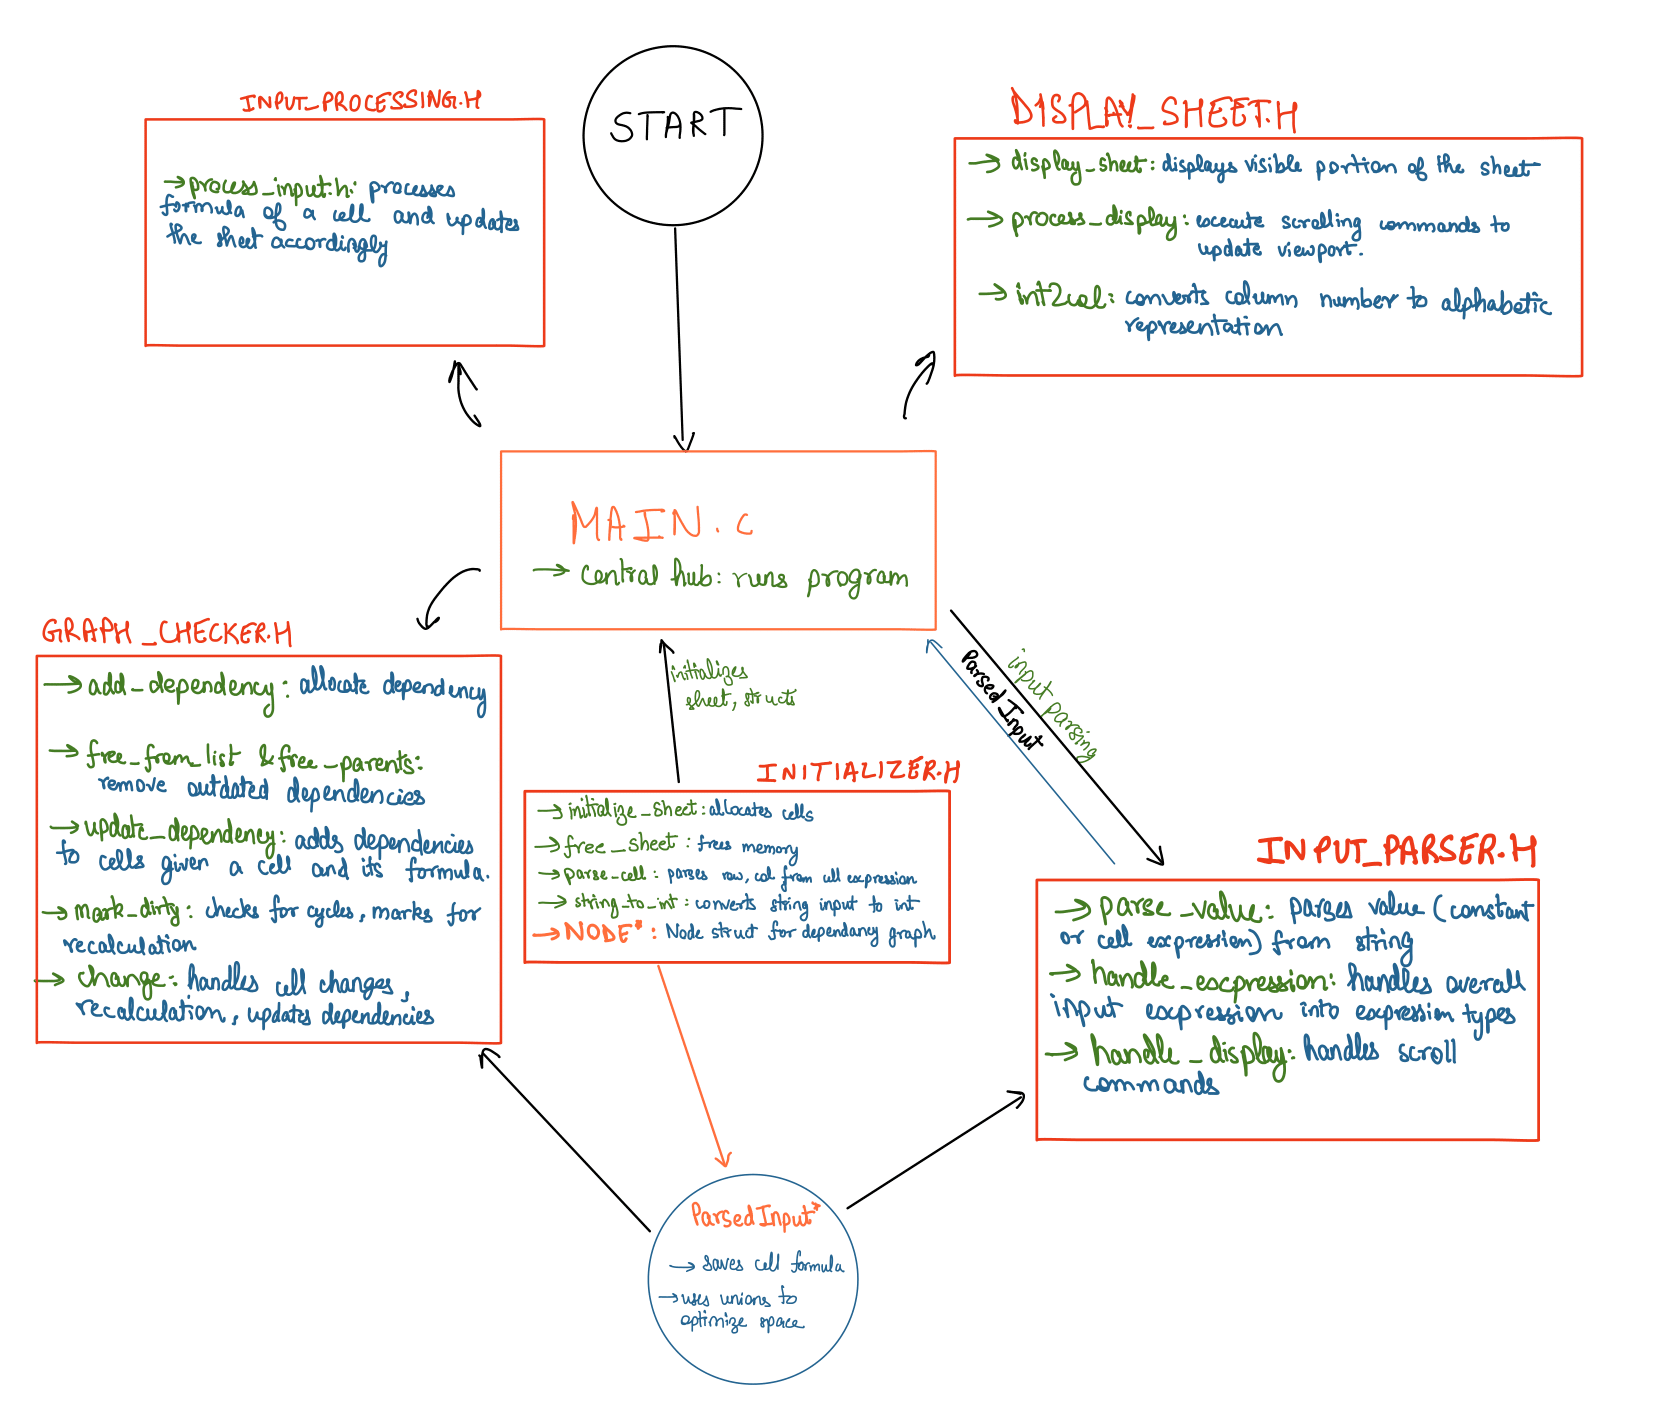
\includegraphics[width=\textwidth]{diagram.png}
    \caption{Overview of Program Structure}
\end{figure}

\textbf{Explanation of Diagram:}
\begin{itemize}
    \item \textbf{Files}: Highlights core modules such as \texttt{main.c}, \texttt{graph\_checker.h}, and \texttt{display\_sheet.h}.
    \item \textbf{Data Structures}: Includes \texttt{ParsedInput}, and \texttt{Node}.
    \item \textbf{Functions}: Displays key workflows, including input parsing, dependency graph traversal, and rendering.
\end{itemize}

\end{document}